\section{Results and Analysis}\label{sec:simulations}
The specifications are verified by comparing simulations results with the expectations. The goal is to verify a correct functioning system, however due to unexpected simulation errors this is not possible. The thick-oxide transistor models in the level shifter cause a simulation crash, therefore the rest of the system is tested with ideal level shifters.
While providing a one tone signal, a transient response of the output power is simulated see Fig.~\ref{fig:Vout_one_tone}.
Next, a DFT of the output voltage is simulated to see the spectral content of the one tone model. To simulate such a DFT the simulation duration should be chosen wisely, an integer number multiple of the period time, otherwise a single tone will not be shown as a single frequency in the spectrum. The simulation time is 256ns (512 LO periods) and the first 15 periods are neglected to filter out settling issues. To fit exactly 11 data periods in this timespan the data frequency should be 42.97 MHz. In Fig.~\ref{fig:DFT_one_tone} shows the 2 GHz carrier frequency and the third and fifth harmonic.
\begin{figure}[h] 
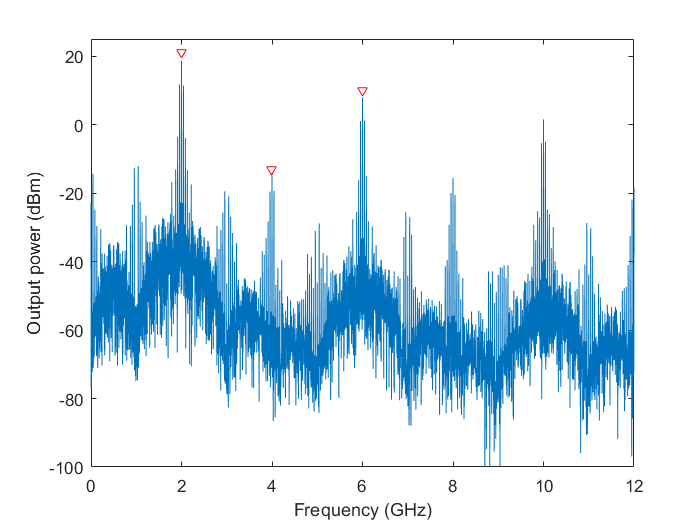
\includegraphics[width=0.5\textwidth]{DFT_one_tone.png}
\caption{The output power spectrum of a single tone test at 42.97MHz.}
\label{fig:DFT_one_tone}
\end{figure}
Furthermore, a two-tone test is simulated. The period time of the second tone fits 14 times in the simulation time, which means that the data frequency of the second tone is equal to 54.69 MHz see Fig. ~\ref{fig:Vout_two_tone}. A two-tone test is useful test the linearity of the DAC, non-linear behaviour generates intermodulation products at the output of the DAC. The power of these intermodulation products should be low, because they interfere with the modulated data tones. Especially the third intermodulation product (IM3), because the IM3 frequencies are very close to the fundamental frequency (at $2f_2-f_1$ and $2f_1-f_2$). It is almost impossible to filter the IM3 noise out of the output signal, therefore it is better to prevent creating IM3 noise. There are more options to express the amount of IM products. For example the spurious-free dynamic range (SFDR) describes power of the fundamental signal to the strongest spurious signal at the output, which is in this case the IM3. Whereas IMD3 describes the difference of the fundamental signal and the IM3.
The spectral constant visualised in Fig.~\ref{fig:DFT_two_tone} shows the 2 GHz carrier frequency and the modulated signals around it. Also the IMD3 is visualised, for these two input signals an IMD3 of 22.59 dBc is measured.
\begin{figure}[h] 
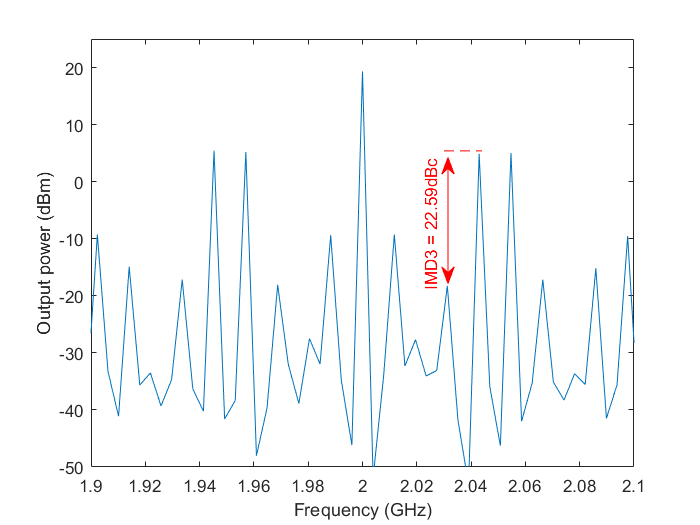
\includegraphics[width=0.5\textwidth]{DFT_two_tone.png}
\caption{The output power spectrum of a two-tone test (42.97MHz and 54.69MHz) shows an IMD3 of 22.59 dBc.}
\label{fig:DFT_two_tone}
\end{figure}
%In addition a frequency sweep of the input signals shows the IMD3 at different bandwidths. In this simulation a constant distance between the input signals is maintained. Results are shown in Fig.~\ref{fig:IMD3}
%\begin{figure}[h] 
%\includegraphics[width=0.5\textwidth]{IMD3_sweep.png}
%\caption{The IMD3 at several bandwidths.}
%\label{fig:IMD3}
%\end{figure}

